\documentclass[a4paper,12pt]{article}
\usepackage[utf8]{inputenc}
\usepackage[top=2cm,bottom=2cm,left=2cm,right=2cm]{geometry}
\usepackage{parskip}
\usepackage{fancyhdr}
\usepackage{graphicx}
\usepackage{hyperref}
\usepackage{listings}
\usepackage{multirow}
\usepackage{dtklogos}
\usepackage[usenames,dvipsnames]{color}

\definecolor{det}{gray}{0.4}

%\newcommand{\revision}{1.0}
%\newcommand{\toast}{2.0.0}
\newcommand{\auth}{Jaci R Brunning}
\newcommand{\editdate}{23rd October 2015}

\newread\toastrevread
\openin\toastrevread=chk/revision.dat
\read\toastrevread to \revision

\newread\toastverread
\openin\toastverread=chk/toast.dat
\read\toastverread to \toast

\newread\toastverread
\openin\toastverread=chk/checksum.dat
\read\toastverread to \checksum

\hypersetup{
	pdfauthor=Jacinta R Brunning,
	pdftitle=Toast API - Whitepaper
}

\pagestyle{fancy}
\lfoot{Toast API Whitepaper}
\rfoot{\thepage}
\cfoot{Revision \revision{} (Toast \toast)}

\setcounter{tocdepth}{4}
\setcounter{secnumdepth}{4}

\lstset{frame=tb,
  aboveskip=3mm,
  belowskip=3mm,
  showstringspaces=false,
  columns=flexible,
  basicstyle={\scriptsize\ttfamily},
  breaklines=true,
  breakatwhitespace=true,
  tabsize=3
}

\begin{document}

\huge \textbf{Toast API - Whitepaper}

\normalsize
\begin{tabular}{p{5.5cm}p{12.5cm}}
	\textbf{Toast Version} &
		\toast\\
	\textbf{Whitepaper Revision} &
		\revision\\
	\textbf{Whitepaper Content Hash} &
		\checksum\\
	\textbf{Revision Date} &
		\editdate\\
	\textbf{Authored By} &
		\auth\\
\end{tabular}

\tableofcontents

\newpage

\section{Abstract}
The Toast API (Toast) is the flagship product of OpenRIO, an Open Source organisation designed for the FIRST Robotics Competition (FRC), dedicated to providing free, useful and open solutions to many challenges facing teams. OpenRIO aims to provide accessible, intuitive software for anyone, anywhere, without the software being branded under any specific team number, therefore belonging to the community that builds it.\\

The Toast API is a fully open-source and modular robotics framework wrapping around the official WPILib library provided by WPI for the FIRST Robotics Competition, and applying patches where needed to ensure the robot environment runs as smoothly and as efficiently as possible. As Toast wraps around WPILib, programmers gain a powerful and familiar experience when interacting with the robot, and with the addition of Toast's utilities, it is a wonderful platform for programmers to develop on regardless of their skill level or previous experience.\\

The purpose of this whitepaper is to outline and discuss why and how Toast works, why and how the framework is deployed and distributed, as well as some of the deviation from the standards of the WPILib library to better suit a modular environment. 

\newpage

\section{Rationale}
The Toast API was developed with the intention of creating a powerful, modular and familiar framework for FRC Developers to use in their own projects or team robots. To achieve this, the rationale is broken down into a number of subcategories:

\subsection{Modularity}
Modularity is the keystone of the Toast API. Toast is designed to be modular in both its internal code structure and its loading of external code and resources. This modular design revolves around the Toast core, with external resources such as Modules and User Libraries can be swapped in and out. This allows for an infinite combinations of configurations and modules, while still maintaining the common Toast Core to ensure a unified environment for all modules to interact on. In this sense, Toast acts as a boilerplate framework for developers to develop their code on top of and ensure it will work on all platforms. The aim of this modular and boilerplate design is the hope that teams will adopt this as a standard, allowing teams to share their code and inspire collaboration throughout the FIRST community.

\subsection{Accessibility}
The Toast API is designed to be used by anyone, anywhere no matter their technological or robotics skill level or background. To achieve this goal, we aim to provide clear, transparent and descriptive documentation with open source code. Documentation provided covers every method and the Toast Wiki is undergoing constant additions and modifications to make it as clear as possible.\\

We have made the decision to migrate away from the Eclipse Plugins that are used by WPILib to deploy a robot program in favour of creating our own Gradle plugin known as GradleRIO to enable easy deployment and accessibility to all platforms, be it Mac, Windows or Linux, as well as different IDEs such as Eclipse or IntelliJ IDEA. The design of GradleRIO has been such that it can run anywhere, and provides all the same (and more) functions present in the official Eclipse plugins, as well as working for the most-recently published version of WPILib automatically. The combination of GradleRIO and the Toast API as a whole is designed to be simple to use, but also enable more advanced users to take advantage of the tools at their disposal by giving them full control. \\

The main reason and philosophy for this level of accessibility is simple: Diversity. FRC is a worldwide competition, and the programmers within the program have a wide variety of skill levels and experiences. To bring these programmers together in a strive to end the stigma of programming within the Robotics Community, the Toast API was designed to be as simple as possible, while remaining a powerful tool for the experienced. Most importantly, the modular design and philosophy enables less experienced programmers to work together with more experienced programmers to create and achieve great things with their code, helping both each other, their team and the world by sharing their code and encouraging collaboration in the community.

\subsection{Language Choice}
The Toast API was decided to adopt the Java Programming language. The reasoning behind choosing Java over C++ or other \textit{(unofficial)} languages is because of the behaviour of the Java Virtual Machine (JVM) and the way it loads classes and deals with objects. The JVM is a largely useful framework that expands much further reaches than just the Java Language, providing control and management that are unrivaled by C++ and other solutions such as Python.\\

The Java Language was chosen as the primary development language over any other JVM language (such as Groovy, Clojure or Scala) to set an example. Not only is Java an official language in regards to FRC, but many teams writing modules will be likely to choose Java on the JVM platform due to familiarity and the wealth of resources available. We decided to write Toast in Java to set a clean example for these people, as teams who choose to use other languages such as Scala or Clojure are likely to have a good deal of understanding about the interoperability in the JVM bytecode between the languages.\\

The JVM was chosen over other solutions for multiple reasons. At first we investigated the possibility of C++, however we deemed it unlikely as it's not a language that is easy to pick up for new programmers and doesn't provide the class-loading flexibility of the JVM. The RobotPy project was another option, but its unofficial support by FRC lead us to believe that it wouldn't be suitable to build a framework on top of. Other languages were also investigated such as the Ruby runtime under both MRI and JRuby, but were dismissed due to complexity and unnecessary bloat on the RoboRIO. We finalised the decision to use Java by seeing that the JVM could run multiple languages natively such as Scala or Clojure, and interpreters could be used in optional modules for language support such as Ruby, LUA or even Python. The JVM Platform was deemed to be the most flexible and reliable for the solution, as well as catering to all skill levels.\\

To utilize the JVM in the Toast context, we apply patches to WPILib's code in certain circumstances such as simulation where the behaviour needs to change. Additionally, the ClassLoader allows for external JAR files (such as modules) to be loaded and instantiated without any issues. This enables modules to be prepared and instantiated natively into the JVM.\\

As mentioned, languages such as Clojure, Scala and Groovy can all be loaded into the JVM. Best of all, they are interoperable, allowing them to run all at once with the common bytecode, with full access to each other, Toast and the entire java runtime. Other languages such as Ruby or LUA can also be interpreted by the JVM using externals libraries. Additionally, Toast comes with inbuilt JavaScript support for on-the-fly scripting and other applications, thanks to the Java Nashorn API that is included with JDK 8 and above. This enables for a large variety of code that can be used by programmers to fit their needs.

\subsection{Deviation}
WPILib was not designed to be a modular framework, and as such, some patches had to be made to ensure that modules are loaded smoothly and do not conflict. Because of these modifications, we have to deviate slightly from the design and conventions set forth in WPILib.

\newpage

\section{Components and Entities}
The Toast API contains many entities, both internal and external, that are used to take an organised and object-oriented approach to loading code and managing your Robot Program and Modules. The purpose of this section is to define and briefly outline the purpose of each entity and the roles they play in Toast's loading and processing phases.

\subsection{Modules}
\textbf{Modules} are jar files containing compiled bytecode compatible with the JVM. These jar files have a class that extends ToastModule in order to be recognised as a module and thus loaded into the classpath and instantiated when Toast's initial setup is complete to give the Module access to the Robot Environment and start executing its code.

\subsection{Core Modules}
\textbf{Core Modules} are similar to Modules, but are loaded during Toast's initial setup and before WPILib is loaded and started. Core Modules follow a slightly different implementation over Modules, with methods relating to initialization without specific hooks or superclasses. Core Modules are designed to have an effect on Toast's loading process, or to execute code that is required before Patching, WPILib and other, non-vital init tasks. This gives Core Modules a large amount of control over the Toast Loading Lifecycle. 

\subsection{JavaScript Modules}
\textbf{JavaScript Modules} are similar to regular Modules, but are instead written in JavaScript and are packaged to be loaded into Toast's Nashorn Engine. JavaScript modules often have a larger overhead, but are commonly used for quick modules. JavaScript can also be loaded without a module for quick scripts stored in their source form, enabling for quick editing, prototyping and coding.

\subsection{External Libraries}
\textbf{External Libraries} are non-module jars that are loaded into the classpath after WPILib and Core Modules, but before regular modules. This enables libraries such as Apache Commons or Guava to be loaded without wasting time searching for a non-existent ToastModule class. In a sense, these are a sort of 'dumb-module', where nothing is instantiated, just added to the classpath to be used later.

\subsection{Load Phase}
A \textbf{Load Phase} is one of 8 phases in the Toast loading lifecycle. These phases indicate what Toast is currently loading, such as Core Modules, Modules, WPILib, Prestart or Start. This makes debugging in crash logs or console logs really simple, as they are clearly indicated in the log file.

\newpage

\section{Lifecycle}
Toast is modular in both the externals and internals. In this section we will be discussing the Toast Loading lifecycle and the role each member plays to ensure reliability, stability and efficiency.

\subsection{Actors}
Toast splits its purpose into actors. An actor is a purpose that code is used for. Actors are spread throughout the lifecycle, but each actor fulfills a different purpose in ensuring the Robot is kept healthy and running perfectly. Toast is split into four (4) main actors. Please keep in mind that actors are not explicity defined in the Toast source files, but are used as an analogy for explanation about how the Toast Ecosystem works.

\subsubsection{The Bootstrap}
The Toast Bootstrap acts as Toast's launchpad. This is where Toast is loaded, and vital utilities such as Command-Line parsing, Logging and Crash Handling utilities and other tools are setup before any externals are loaded. Because Logging and Crash Handling frameworks are setup here, the Bootstrap is often regarded as the most stable portion of the Toast lifecycle, and is therefore mostly non-configurable.  

\subsubsection{The Modules}
The Modules are pieces of code written by programmers specifically for Robot Control. Module Actors are responsible for Module discovery, preparation, and finally, loading. This includes verifying the main class for each module, handling any dependency branches as well as ensuring Core Modules are treated appropriately. This Actor also ensures the appropriate hooks are provided to the module for launch. Additionally, any External Libraries are loaded and added to the classpath by this actor.

\subsubsection{The Non Vitals}
The Non-Vitals in the Toast Lifecycle are the utilities that Toast loads that aren't necessary vital to the loading process, but still used. This includes things such as the ClassPatcher, Simulation GUI and WPILib itself. This actor is responsible for loading of Toast's utilities in an orderly and efficient manner.

\subsubsection{The Directors}
The Directors are actors that are used to 'direct' modules and their components. The most prevalent director is the Toast class. The Toast class extends WPILib's RobotBase and handles WPILib's robot hooks such as prestart and start, as well as state tracking. The Toast class and StateTracker class delegate robot status and state events to all listening modules to ensure all modules get the message and can act appropriately. The Heartbeat, ASync and Network Delegate systems are also recognised as directors.

\subsection{Loading Lifecycle}
The loading lifecycle of Toast is split into different phases to represent a simple way to debug loading issues and to keep loaded elements separated to maximize organisation and minimize issues. Load Phases are points in the Robot Program that dictate what is currently happening, and make it easy to debug and read the Load Status of the robot to detect potential issues leaving the program unusually slow, or even leading to a crash. The Loading Lifecycle of Toast is best described by the following image.

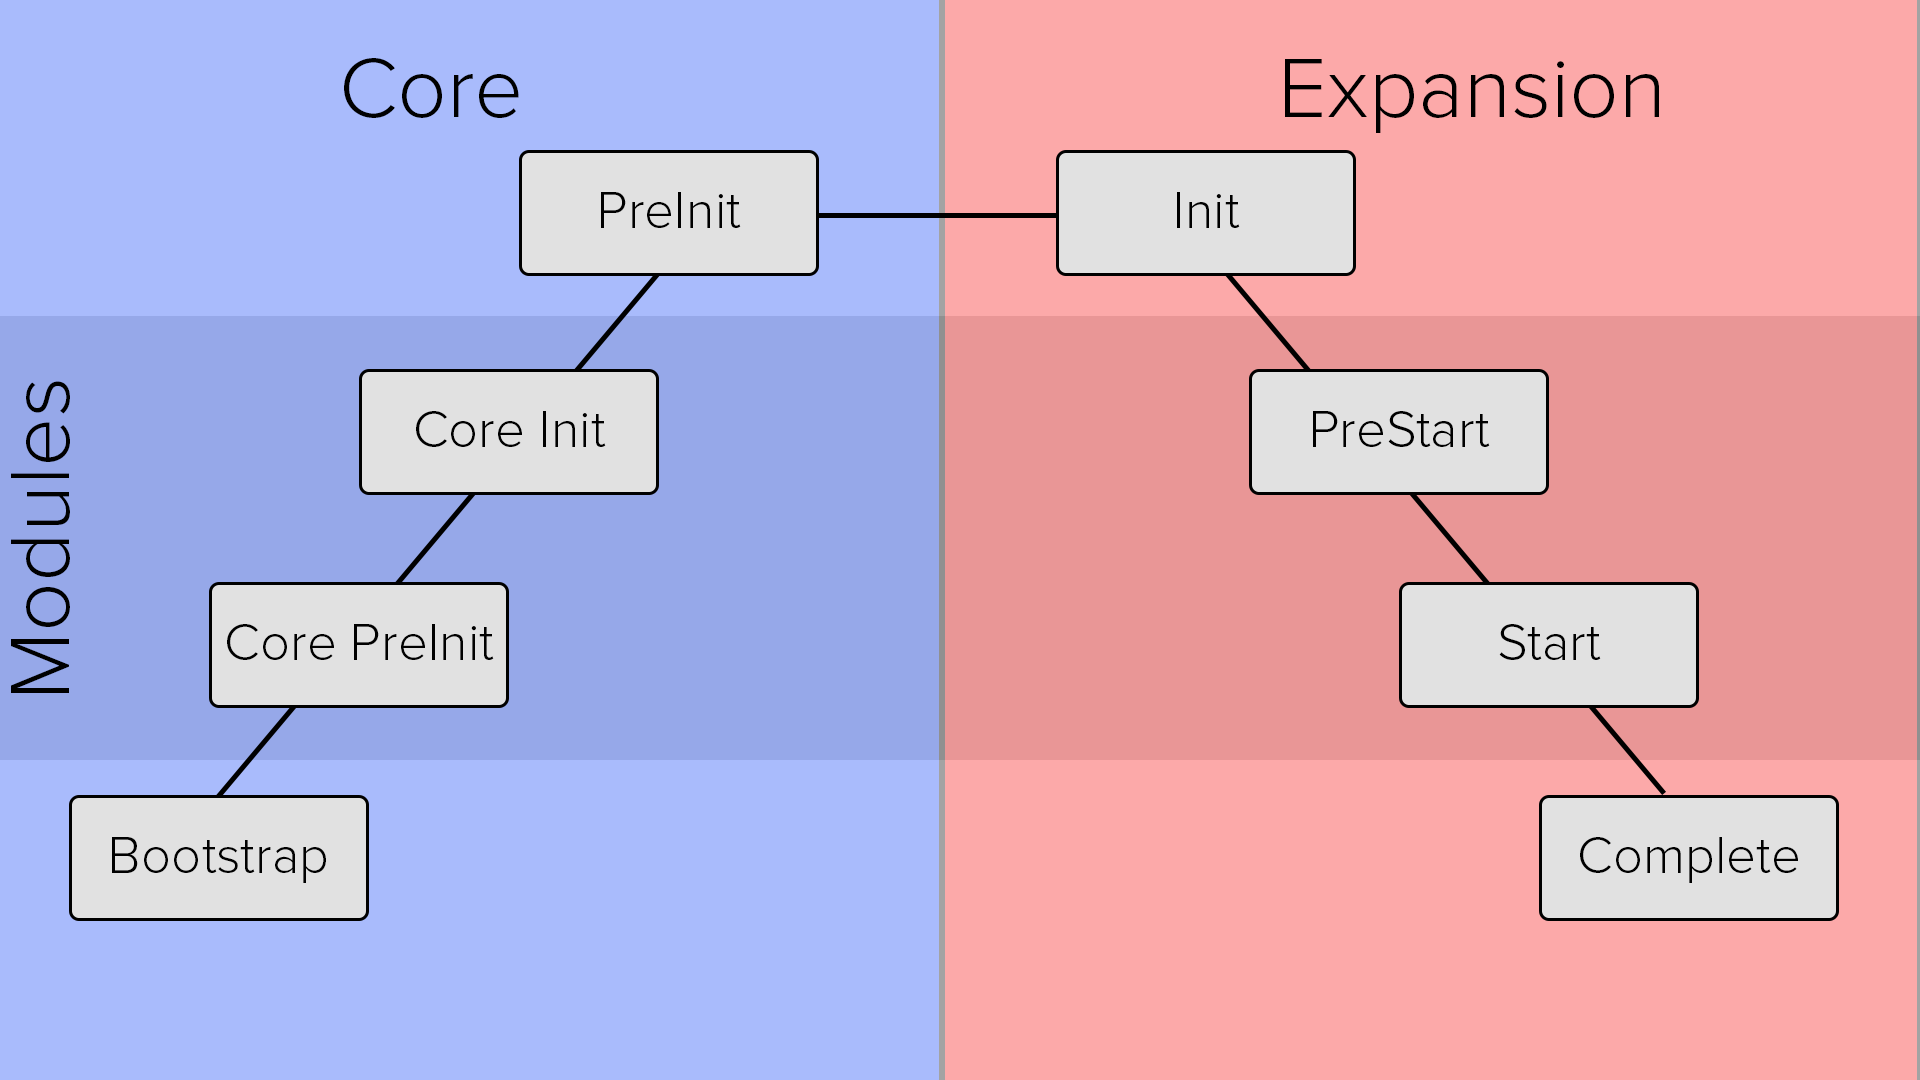
\includegraphics[width=17cm]{img/lifecycle.png}

\subsubsection{Sections}
The diagram above is noticeably split into multiple sections. Each colored section has a specific role, and following are the explanations for each.

\begin{tabular}{p{3.5cm}p{12.5cm}}
	\textbf{Blue (Core)} &
		The Blue (Core) Section contains all the loading that is done before WPILib is initialized, such as module discovery, patching, utility setup and preference loading.\\\\
	\textbf{Red (Expansion)} &
		The Red (Expansion) Section contains everything loaded after or during WPILib. This is where modules are loaded and services start. Most of, if not all of your code is handled in this section.\\\\
	\textbf{Dark (Modules)} &
		The Dark (Modules) Section is the subset of Load Phases in which modules interact. For example, Core Modules and regular Modules all undergo discovery, initialization and setup in the phases encapsulated in this dark section. Cross-Sectioning \textit{Modules} and \textit{Expansion} will yeild the section that most Modules operate in.\\\\
\end{tabular}

\subsubsection{Load Phases}
\begin{tabular}{p{3cm}p{12.5cm}}
	\textbf{Bootstrap} &
		The Bootstrap Phase is where Toast loads the 'bare essentials'. This is where command-line options are parsed, loggers and crash handlers are started, as well as the global blackboard and other vital utilities. This is the most stable section.\\\\
	\textbf{Core Preinit} &
		The Core Preinit Phase serves 2 main purposes, to prepare modules for loading and candidacy, and to load core modules. Modules are searched for and are categorized into Modules or Core Modules. All modules are analysed for candidacy, that is, a base class is present and/or a Manifest attribute is present. Core Modules are initialized here, while regular modules remain dormant.\\\\
	\textbf{Core Init} &
		The Core Init Phase is where Core Modules finalize their loading. Core Modules can now be assured that all Core Modules have undergone basic preinit and thus can communicate between each other.\\\\
	\textbf{Pre Init} &
		The Pre Init Phase is where Toast finalizes loading its utilities. This includes optional utilities such as preferences, but also loads things vital to loading WPILib such as the Class Patcher and Simulation if required.\\\\
	\textbf{Init} &
		The Init Phase is where WPILib is loaded. This phase is largely outside of Toast's jurisdiction, except for classes that have been patched by Toast. WPILib will continue to load Toast's RobotBase class when hardware configuration (or simulation abstraction) is available.\\\\
	\textbf{Pre Start} &
		The Prestart Phase, much like WPILib, is where preliminary setup is done before the Robot is marked 'ready'. This is where modules that are valid candidates are finally instantiated, and then put through their 'prestart' phase, which is intended to do the bulk of module setup that doesn't require other modules. After this phase, the robot is marked as 'ready to go'.\\\\
	\textbf{Start} &
		The Start Phase is where Modules finalize their setup. At this point, all modules have gone through 'prestart', which means they are free to communicate to one another. This service also begins networking services. By this time, the Robot is fully setup and ready to rock.\\\\
	\textbf{Complete} &
		The Complete Phase recognises that all Robot Setup is complete and is now ready to begin transitioning into the looping operation of the Robot. This is where the StateTracker is started and all Robot logic is now state-based.
\end{tabular}

Load Phases are separated as opposed to one bulk "setup" period is to ensure that modules have a guaranteed idea of when things are ready to be interacted with, as well as for easy debugging, as each load phase is indicated by the Thread Name in the logger. This also makes it simple to discuss how Toast works behind-the-scenes.

\subsection{Robot States}
\textbf{Robot States} are Toast's way of handling the various modes the robot can be in during competition, practise or testing. These states are the well-known Disabled, Autonomous, Teleop and Test modes as seen in the Driver Station or the familiar IterativeRobot baseclass. Since no two states can occur at the same time (no superpositions), all the states are stored in an Enumeration for easy access.\\

State Tracking is done by the appropriatly named "StateTracker" class. Modules can subscribe or register on the bus to be alerted when the Robot switches (transitions) or ticks on a State. These transition and ticking states are used to control the way the robot interacts. Tickers are listeners that are called periodically with the regular timing loop of the IterativeRobot class. This ensures all modules get access to basic robot function.

\subsubsection{Transition}
\textbf{Transition} is the action produced when the Robot migrates from one operational state to another, for example, the transition between Disabled and Autonomous. The 'StateListener' interface provides hooks for listening for this transition, providing two parameters, the new state and the old state. These state parameters are also stored statically in the StateTracker class. The purpose behind this is to allow actions to be triggered when a state is stopped as well as started, for example, stopping autonomous when we switch to teleop or disabled abruptly.

\subsubsection{Ticking}
\textbf{Ticking} is the action produced on a periodic basis. This is similar to the 'autonomousPeriodic' or 'teleopPeriodic' methods that most robot base classes overload in order to function. Toast abstracts this to a listener system so you can use it if you want, or use multiple if your module requires it. The ticking function is called with a 20ms interval, or whenever new control data is available. This is in-line with WPILib's implementation on their IterativeRobot class. This is used for periodic action such as moving motors based on sensor input.\\

The basic rationale behind this operation is because of modules. Modules can choose to subscribe if they want to, implement a ModuleBase class that does it automatically, or subscribe more than once, depending on what the module requires. This creates a modular and customizable workflow for modules working with states.

\newpage

\section{Logging and Debugging}
Debugging is one of the most difficult things to do effectively on a remote host (such as the RoboRIO), especially for inexperienced programmers. To solve this issue, Toast provides a fully featured logging framework with support for file logging as well as to Standard Out. Additionally, Live-Debugging tools are provided and a Crash Handler has been crafted to ensure that any crashes that occur on the Robot are handled properly and able to be read easily.

\subsection{Logging}
Toast provides a fully featured logging framework to ensure any messages that are to be sent out by Toast and its modules can be accessed easily and are saved to file to be retrieved later. In order to provide a comprehensive output, Toast formats its logs in a very specific way, but will also channel STDOUT to file if you don't want to use the Logging format. STDOUT and STDERR are stored in their respective files, as well as a combined file. The general format used by log messages is depicted below:

\hspace{2cm} \textit{[date-time] [logger-name] [thread-name] [level] Message}

Both the Date-Time and Thread-Name portions of the log message are optional, and are defined in the Logger class' constructor.

\subsubsection{Log Levels}
The Log-Level is one of four (4) options. These options exist to categorize log messages in terms of urgency.

\begin{tabular}{p{2cm}p{12.5cm}}
	\textbf{Info} &
		The \textbf{Info} log level is used for standard logging and directs to Stdout. This is used for general-purpose logging that shouldn't cause any alarm.\\\\
	\textbf{Warn} &
		The \textbf{Warn} log level is used for logging low-level errors that should be seen but aren't necessarily that important. This level goes to Stderr.\\\\
	\textbf{Error} &
		The \textbf{Error} log level is used for high-level errors that don't cause the robot to crash. This is usually used if a motor or sensor is not connected, or if an exception is called.\\\\
	\textbf{Severe} &
		The \textbf{Severe} log level is used for high-level errors that do cause a crash. This is usually seen before the Robot is shut down in the event of an uncaught exception or robot software crash.\\\\
\end{tabular}

Each Log Level Stream are split between a File, a Networking Socket (if a client is connected), and the Stdout and Error streams. This allows for logs to be saved to file to be read later and sent to programmers to fix their bugs fast. Crash Log excerpts and full logs are backed up to file to be read from later.

\subsection{Crash Handling}
The Crash Handling in Toast is a means by which developers can get helpful insights into what caused the robot to break. In Toast, Crash Logs are formatted, have extra information and are even saved to file with a timestamp and full session log of the robot. This data is easily accessible through SSH, SCP or even USB Devices, as well as other methods. Below is a sample crash log from a Toast Session.

\begin{lstlisting}
**** CRASH LOG ****
Your robot has crashed. Following is a crash log and more details.
This log has been saved to: D:\Programming\FRC\OpenRIO\Toast\run\toast\crash\crash-2015-07-05_06-48-37.txt
 ________     __  ____       ____  __
((       )   / / / / /_     / __ \/ /_
||  x x  |  / / / / __ \   / / / / __ \
||   ^   | / /_/ / / / /  / /_/ / / / /
\\_______/ \____/_/ /_/   \____/_/ /_/

java.lang.Exception: Invoked Debug Crash
    at jaci.openrio.toast.core.command.cmd.CommandInvokeCrash.invokeCommand(CommandInvokeCrash.java:35)
    at jaci.openrio.toast.core.command.CommandBus.parseMessage(CommandBus.java:78)
    at jaci.openrio.toast.core.command.CommandBus$1.run(CommandBus.java:167)

Crash Information:
    Toast:
        Toast Version: 2.0.0
        Loaded Modules:

    Environment:
            Toast: 2.0.0
             Type: Simulation
              FMS: false
               OS: Windows 8.1 6.3 (amd64)
             Java: 1.8.0_25 (Oracle Corporation)
        Java Path: C:\Program Files\Java\jdk1.8.0_25\jre
          JScript: Supported (Nashorn)


*******************
\end{lstlisting}

As seen, all this data is formatted nice and cleanly, with all the information about the Toast Environment, Robot Status, Backtrace and Loaded Modules being presented in an easy to read format. Additionally, modules can put their own data in the Robot Crash Log using the class CrashInfoProvider, which will append it to the end of the log in the same style of the `Environment' provider.

\subsection{Debugging}
As a part of the GradleRIO build system plugin, a method by which a robot program can be remotely connected to and live debugging and code hot-swapping support. The Java Language comes with a debugging server inbuilt which can be triggered by a command line argument, and then connected to by an IDE to inspect code using breakpoints as it runs, as well as editing code on the fly. 

In order to get this debugging server on the RoboRIO, we use a set of gradle tasks known as `rioModeRun', `rioModeDebug' and `rioModeHybrid'. All debugging modes are launched on port 5910 through dt\_socket and can be accessed by Eclipse and IntelliJ IDEs. Each mode is described briefly below.

\subsubsection{Run Mode}
\textbf{Run Mode} is the standard mode that the RoboRIO runs in. No debugging server is launched, but instead the code is just run.

\subsubsection{Debug Mode}
\textbf{Debug Mode} is a mode by which a debugging server is launched, but the RoboRIO's code will not start until a remote debugger is attached. This means that coe inspection right from the start of the code can be done without any issues.

\subsubsection{Hybrid Mode}
\textbf{Hybrid Mode} is a mode by which a debugging server is launched, but will not wait for a remote debugger. The robot code will execute as normal, and will accept a debugger to be connected at any time. This is useful for competition use.

\subsection{Environment}
Since Toast is a cross-platform framework, it is helpful to know what environment the robot is running on. Toast will gather information about the Robot's environment such as OS, Toast Version, Environment Type, Java details and FMS connectivity. All this data is analysed and can be accessed by any module. This data is printed in the event of a crash, under the Environment CrashInfoProvider.

\newpage

\section{Configurations}
Configurations are Toast's way of enabling a user to manipulate data in a module without having to recompile or build their own support. Configurations are handled by the ModuleConfig class and are stored to file in JSON format. The user can manipulate these configuration files to suit their own needs. Below is the standard configuration file for Toast itself.

\begin{lstlisting}
{
	"delegate":{
		"logger":{
			"password":"",
			"algorithm":"SHA256"
		},
		"command":{
			"password":"",
			"algorithm":"SHA256"
		}
	},
	"robot":{
		"name":"My Robot Name",
		"team":0000,
		"desc":"This is my Robot!"
	},
	"security":{
		"policy":"STRICT"
	},
	"optimization":{
		"gc":{
			"time":30,
			"enabled":false
		}
	},
	"threading":{
		"pool_size":4
	},
	"javascript":{
		"autoload":["main.js"]
	}
}

\end{lstlisting}

Configurations are designed to be user-friendly and transportable. Any keys not already present in the Configuration are automatically added to the file.

\newpage

\section{USB Mass Storage}
Toast has made the decision to take advantage of the 2 USB Ports provided on the RoboRIO that can accept any USB peripherals, including USB Mass Storage drives (pen drives). USB Drives can be utilized by Toast to increase the internal file system storage, or to use as a transportable platform for carrying modules, configurations, and other data.

Every USB Drive used by Toast has a mandatory toast\_autorun.conf file. This file contains the configuration for the USB device itself, including how the USB behaves, what its name is, and where the directories are stored. USB Configs can be generated by the `usb generate' command, or by the \url{http://dev.imjac.in/toast/usb/} site. An example is seen below:

\begin{lstlisting}
{
    "toast": {
        "device_name":"Team_####_USB_Device",
        "directory": "toast",
        "dumps": "toast_usb_dumps",
        "override_modules": false,
        "concurrent_modules": true,
        "accept_logs": true,
        "priority": {
            "config": 0,
            "filesystem": 0
        }
    }
}
\end{lstlisting}

The most common use of USB Mass Storage is Concurrent Modules. The Concurrent Modules setting will allow for modules and libraries on the USB Device to be loaded side-by-side with those on the RoboRIO (if any exist). This means teams can carry around modules on a handy USB device to plug into the RoboRIO and have their code instantly work. 

The Override Modules mode is used to completely disable the RoboRIO's internal module storage in favour of those on the USB Device. This is commonly used as a form of `code backup', should code stop working during competition. Modules on the USB Device will be loaded instead of those on the RoboRIO, making it useful for debugging or simply as a hotswap for competition, potentially for different robot configurations. This can also be used as a backup USB for other teams, or if a team shows up to the competition without fully working code. This means teams can share their resources and build a better competition all-together.

USB Devices can also be used as a way to keep track of logs. Because of the RoboRIO's small storage space, only the most recent logs are stored (or saved if they have crashed). In order to save ALL logs with a timestamp, the accept\_logs option can be toggled to true to store all the Log outputs onto the device to be read from later. 

The Priority System is used to judge what USB device (or internal storage) is to be used for what purpose. The device with the highest priority.config option (internal storage is priority 0) will be used to store and read from Configuration Files. The device with the highest config.filesystem option will be used to store and read files saved by modules, such as event logs or custom data. The priority system takes an organized approach to File management among multiple file systems.

All the Toast data on the RoboRIO's internal storage can be dumped to a USB device (or loaded) using the `usb dump' and `usb load' commands. These enable Crash Logs, module files, configurations and just about all the Toast data on a RoboRIO to be dumped to a USB device and restored at a later date. This makes the USB device an extremely powerful tool in the Toast ecosystem.

\newpage

\section{Command Bus}
Toast comes with a simple CommandBus implementation. The Command Bus is an interface that takes in data from the Command Line (or a remote console) and passes it to Toast or the appropriate module to be processed. This means modules can register their own commands that invoke and action when used.

Toast has a handful of included commands that can monitor Threads, Reload Configurations, On-The-Fly Scripting, Profiler Readouts, and even Invoking Debug Crashes. The Command Bus is open to any module to use and can be an extremely powerful tool.

\subsection{Helpables}
Some Commands may choose to implement IHelpable. By implementing IHelpable, they can provide a `help' message that will be displayed to the user. This makes Commands intuitive and easy to pick up by users.

\newpage

\section{Threading and Async}
The Toast API provides utilities to aid in the Threading process. As Multithreading is something hard to get right and can easily get out of hand, especially in a Robotics environment, Toast provides built-in support for Asynchronous Background Tasks on a managed Thread Pool.

Modules submit work to the Async class to execute when resources become available. The Async class has 4 working threads by default, but that can be configured in the Toast.conf configuration file. Work is executed on a \textit{First In - First Out (FIFO)} basis, where the sooner you submit the work, the sooner it will be completed.

The Async class will continually fetch work from the queue for each thread. Since work is executed when available, there is no guarantee when the work will be completed. Due to this, the Async behaviour is usually used for background tasks or callbacks. Furthermore, because Async is set up as a Thread Pool with limited working threads at any given time, largely Time-Consuming tasks such as Network I/O or Thread.sleep calls should not be present in an Asynchronous Task, as they bog down the system for everyone. If you require the full power of an Async class, you can create a new instance of it and dedicate it to your own tasks.

The Async Thread Pool requires modules to be weary of how much time their task takes up, as Toast will not automatically kill threads if they are sleeping (blocking) for too long. The Async bus is to be used for background tasks that are not time-specific for when they are executed.

\newpage

\section{Networking}
The Field Management System (FMS) for FRC restricts the amount of ports any given robot and driver station can have open for communication. These ports, \textit{(5800 -- 5810)} restrict the amount of ports a robot can have open, and therefore can cause conflicts between modules that require networking support. To solve this \textit{(for TCP connections)}, Toast comes bundled with the NetworkDelegate API, another product of OpenRIO designed to share an infinite number of servers on a limited number of ports. 

Network Delegate requires sockets requesting connection to the RoboRIO to make an initial request to the Master port \textit{(5805)}. The Master Port will take in the name of the service the client wishes to connect to and delegate it a port between the range of 5806 -- 5810. The client then disconnects from the master socket and reconnects to the delegated socket with their details. This socket is then verified and the raw socket object is passed to the Module running the delegate server. This gives modules access to the raw socket object as if it were a regular TCP Server, but without the headache of clashing with other modules that happen to use the same port.

All of NetworkDelegate is handled by the SocketManager class, where Modules can create their own Delegate Servers and host them on the RoboRIO, ready for clients to connect to. Delegate Servers also have an optional password, which can be hashed with SHA256, MD5 or SHA1. This provides basic security for the Delegate Server. 

Delegate IDs are unique to the module or service they belong to, so an ID such as `modulename\_delegate' is not uncommon. This is what the client sends when they wish to connect. Network Delegate has a library for Java clients, however the spec is fully documented for those who wish to implement it in their own language. More about Network Delegate can be seen on the GitHub project under OpenRIO.

Ports 5800 -- 5804 are untouched by NetworkDelegate, and are kept available for services \textit{(such as the WebUI with HTTP)} that require a specific protocol and therefore can't conform to the NetworkDelegate spec. While you are free to use these ports, it is not recommended as you can run into issues with Socket Port collisions. If you're able to, NetworkDelegate is the best way to go to ensure smooth robot operation over the network.

\newpage

\section{Language Integration}
Toast is written in Java, the staple language of the popular JVM. Because of the JVM's capabilities, Toast is able to support many languages out of the box.

\subsection{JavaScript}
Java Version 8 and above come packaged with the Nashorn JavaScript runtime environment by Oracle. Nashorn provides support for JavaScript interpretation on the JVM, and full interoperability between the two. JavaScript can be loaded on-the-fly using the `script' command, or loaded from packaged JavaScript modules \textit{(.jsm)}, or even loaded from user-created scripts under the Toast directory stored in JavaScript source files \textit{(.js)}. JavaScript has full access to the JVM's capabilities, and Toast provides a framework by which code written in JavaScript can interact with code written in Java, as well as providing the hooks to make this process simple and familiar to the language. Writing code in JavaScript can be useful for quick on-the-fly maintenance, quick scripting and prototyping, and even deployment of full modules. 

Although JavaScript interpretation is noticably slower than native Java Bytecode, it is still a powerful tool for those who want to use it. To avoid taking up a lot of time loading the JavaScript engine and included libraries, Toast will start JS loading in a new thread, and only modules that require JS interpretation will take the time to wait for it to be initialized. This minimizes the effect of the Nashorn engine on the Toast loading process.

\subsection{JVM Languages}
Since Toast runs on the JVM, there is support for other languages that also run on the JVM. JVM Languages are interoperable, as down to the core they are all JVM bytecode. Languages such as Groovy, Scala, Kotlin and Clojure can all be run alongside Toast and work natively with no issues, with access to everything, including Toast, WPILib and any modules loaded. JVM Languages can be extremely powerful, as each provides its own advantages to its application in a Robotics environment. 

\subsection{Interpreted Languages}
Interpreted Languages such as Ruby and LUA can all be loaded into Toast as well, through what's known as Language Support Modules. Language Support Modules are just like regular modules, but come bundled with an interpreter such as JRuby or LuaJ. These interpreters provides hooks to the JVM and Toast/WPILib methods, allowing them access to the underlying framework. While these may not be as fully featured as JVM Languages, they are still very useful and can be configured to be very powerful. JRuby includes support for JVM imports, allowing virtually unlimited access, while LuaJ requires the ToastLua module to provide the hooks. 

\newpage

\section{Dependency Management}
Toast provides ways that modules can manage their dependencies. Most of these methods use soft dependencies. Soft dependencies are dependencies that are optional, and if they are loaded, certain actions will occur. 

\subsection{Branch Model}
The Branch Model is a unique approach to soft dependency management. At the top of your Module file, a @Branch annotation is added. This annotation defines a class and method to load, and a module or class name. If the module or classname is present in the loadpath (that is, it exists and is loaded by Toast), the Class and Method will be loaded and executed. If it is not present, nothing happens. 

The Branch Model provides a way for optional dependencies to act in a unique way, and is often used in conjunction with API classes for modules that are accessed via code.

\subsection{Module Event Bus}
The Module Event Bus uses a listener-emitter system to provide an event-based approach to cross-module communication. Modules register a listener on the Module Event Bus. Whenever an event is raised, the listener is called and the properties of the Event are passed to it. These properties include the target name (this is usually your module name), the action name, and the parameters. It is left up to the listener to decide what events trigger what actions, and so  most listeners often start with the line `if (target.equals("MyTarget"))' to ensure it isn't triggered for events destined for other modules.

The Module Event Bus will only dispatch to listeners that are registered, and so, if the target module is not present, the event will not be captured and therefore nothing will occur. This is mostly used for API calls that do not require a response. The Module Event Bus means that dependencies can be managed completely optionally, and also allows for events to be logged into a history by accepting all targets.

\subsection{@Priority and Method Execution}
The @Priority annotation is designed to be used on the prestart() and start() methods of the ToastModule class and its children. This annotation defines the `priority' of a method execution in the list of modules. The higher this value, the higher priority the method execution is placed in the queue, hence the sooner it will be executed. This allows for modules to define \textit{when} their prestart method will be called.

An example implementation of this would be when depending on a library/api module. The API module would put their prestart() method on the Highest priority, meaning it can complete its setup first out of all the modules. The dependant module would use the Lowest priority, meaning they are \textit{guaranteed} to execute after the API, therefore assuring that the API module will have completed its setup first.

This implementation is extremely useful when using multi-module projects, as execution can be controlled by the modules to their requirements. 

\newpage

\section{The Heatbeat System}
The Heartbeat System is Toast's implementation of a timed loop that occurs \textit{exactly} once every 100ms. This allows for implementations that require a constant `heartbeat' to be triggered at a constant pace.

The heartbeat system keeps track of how long each heartbeat took to execute, and will adjust the next delay accordingly to ensure a 100ms loop as accurately as possible. With this also comes the `skipped beat' implementation. If a heartbeat takes longer than 100ms to execute, the system will `skip a beat' and echo a warning to the logger. Heartbeat Listeners will also be notified of the amount of beats skipped so they can adjust accordingly. Through this implementation, listeners can be assured that they will be triggered at a regular pace.

The heartbeat system is smart in the respect that it will not tick if there are no listeners present. This saves CPU time and ensures the robot does not do anything that it doesn't need to. As soon as a listener is registered, the Heartbeat will start and will continue to run until the robot program has completed. This ensures that resources are not wasted. 

The heartbeat system operates completely independently from the StateTracker, meaning the Heartbeat will continue to pump through any state.

\newpage

\section{Simulation and Verification}
Through the use of the Class Patcher, Toast has the ability to replace WPILib's classes when run in a development environment, or with the -sim command line flag. This allows us to redirect the native HAL (Hardware Abstraction Layer) calls to a GUI to enable the Robot's inputs and outputs to be simulated. This provides an easy and native way for developers to test their code without having physical access to the robot, but still be running the same code on the frontend. If possible, all patching is done to the HAL to ensure WPILib updates don't break the system. 

\includegraphics[width=10cm]{img/sim.png}

Verification is used as a form of `headless simulation'. The GUI is not initialized, but instead the Autonomous and Teleoperated periods are on timed cycles similar to that of an FRC match (15 seconds autonomous, 2:15 minute teleoperated). This allows build systems and continuous integration services such as Travis CI and Jenkins to run tests on the robot program extremely easily. This is denoted by the -verify command line flag.

\end{document}